%%%%%%%%%%%%%%%%%%%%%%%%%%%%%%%%%%%%%%%%%%%%%%%%%%%%%%%%%%%%%%%%%%%%%%%%%%%%
% AGUJournalTemplate.tex: this template file is for articles formatted with LaTeX
%
% This file includes commands and instructions
% given in the order necessary to produce a final output that will
% satisfy AGU requirements, including customized APA reference formatting.
%
% You may copy this file and give it your
% article name, and enter your text.
%
%
% Step 1: Set the \documentclass
%
%

%% To submit your paper:
\documentclass[draft]{agujournal2019}
\usepackage{url} %this package should fix any errors with URLs in refs.
\usepackage{lineno}
\usepackage[inline]{trackchanges} %for better track changes. finalnew option will compile document with changes incorporated.
\usepackage{soul}
\linenumbers
%%%%%%%
% As of 2018 we recommend use of the TrackChanges package to mark revisions.
% The trackchanges package adds five new LaTeX commands:
%
%  \note[editor]{The note}
%  \annote[editor]{Text to annotate}{The note}
%  \add[editor]{Text to add}
%  \remove[editor]{Text to remove}
%  \change[editor]{Text to remove}{Text to add}
%
% complete documentation is here: http://trackchanges.sourceforge.net/
%%%%%%%

\draftfalse

%% Enter journal name below.
%% Choose from this list of Journals:
%
% JGR: Atmospheres
% JGR: Biogeosciences
% JGR: Earth Surface
% JGR: Oceans
% JGR: Planets
% JGR: Solid Earth
% JGR: Space Physics
% Global Biogeochemical Cycles
% Geophysical Research Letters
% Paleoceanography and Paleoclimatology
% Radio Science
% Reviews of Geophysics
% Tectonics
% Space Weather
% Water Resources Research
% Geochemistry, Geophysics, Geosystems
% Journal of Advances in Modeling Earth Systems (JAMES)
% Earth's Future
% Earth and Space Science
% Geohealth
%
% ie, \journalname{Water Resources Research}

\journalname{Journal of Advances in Modeling Earth Systems (JAMES)}


\begin{document}

%% ------------------------------------------------------------------------ %%
%  Title
%
% (A title should be specific, informative, and brief. Use
% abbreviations only if they are defined in the abstract. Titles that
% start with general keywords then specific terms are optimized in
% searches)
%
%% ------------------------------------------------------------------------ %%

% Example: \title{This is a test title}

\title{NCAR release of CAM-SE in CESM2.2: topography and viscosity, middle atmosphere sponge layer diffusion, variable resolution, ....}

%% ------------------------------------------------------------------------ %%
%
%  AUTHORS AND AFFILIATIONS
%
%% ------------------------------------------------------------------------ %%

% Authors are individuals who have significantly contributed to the
% research and preparation of the article. Group authors are allowed, if
% each author in the group is separately identified in an appendix.)

% List authors by first name or initial followed by last name and
% separated by commas. Use \affil{} to number affiliations, and
% \thanks{} for author notes.
% Additional author notes should be indicated with \thanks{} (for
% example, for current addresses).

% Example: \authors{A. B. Author\affil{1}\thanks{Current address, Antartica}, B. C. Author\affil{2,3}, and D. E.
% Author\affil{3,4}\thanks{Also funded by Monsanto.}}
\authors{Peter H. Lauritzen\affil{1}\thanks{1850 Table Mesa Drive, Boulder, Colorado, USA}, and Adam R. Herrington\affil{1}, Han-Li Liu\affil{1}}

 \affiliation{1}{National Center for Atmospheric Research, Boulder, Colorado, USA}


% \affiliation{1}{First Affiliation}
% \affiliation{2}{Second Affiliation}
% \affiliation{3}{Third Affiliation}
% \affiliation{4}{Fourth Affiliation}

\affiliation{=number=}{=Affiliation Address=}
%(repeat as many times as is necessary)

%% Corresponding Author:
% Corresponding author mailing address and e-mail address:

% (include name and email addresses of the corresponding author.  More
% than one corresponding author is allowed in this LaTeX file and for
% publication; but only one corresponding author is allowed in our
% editorial system.)

% Example: \correspondingauthor{First and Last Name}{email@address.edu}

\correspondingauthor{=name=}{=email address=}

%% Keypoints, final entry on title page.

%  List up to three key points (at least one is required)
%  Key Points summarize the main points and conclusions of the article
%  Each must be 140 characters or fewer with no special characters or punctuation and must be complete sentences

% Example:
% \begin{keypoints}
% \item	List up to three key points (at least one is required)
% \item	Key Points summarize the main points and conclusions of the article
% \item	Each must be 140 characters or fewer with no special characters or punctuation and must be complete sentences
% \end{keypoints}

\begin{keypoints}
\item The deadline for submission of the manuscripts to the AGU CESM2 Virtual Special Issue has been extended to 30 September 2020. 
\item enter point 2 here
\item enter point 3 here
\end{keypoints}

%% ------------------------------------------------------------------------ %%
%
%  ABSTRACT and PLAIN LANGUAGE SUMMARY
%
% A good Abstract will begin with a short description of the problem
% being addressed, briefly describe the new data or analyses, then
% briefly states the main conclusion(s) and how they are supported and
% uncertainties.

% The Plain Language Summary should be written for a broad audience,
% including journalists and the science-interested public, that will not have 
% a background in your field.
%
% A Plain Language Summary is required in GRL, JGR: Planets, JGR: Biogeosciences,
% JGR: Oceans, G-Cubed, Reviews of Geophysics, and JAMES.
% see http://sharingscience.agu.org/creating-plain-language-summary/)
%
%% ------------------------------------------------------------------------ %%

%% \begin{abstract} starts the second page

\begin{abstract}
[ enter your Abstract here ]
\end{abstract}

\section*{Plain Language Summary}
[ enter your Plain Language Summary here or delete this section]


%% ------------------------------------------------------------------------ %%
%
%  TEXT
%
%% ------------------------------------------------------------------------ %%

%%% Suggested section heads:
\section{Introduction}
\begin{itemize}
\item development process is not always linear
\item some engineering solutions necessary
\item 
\end{itemize}
%
% The main text should start with an introduction. Except for short
% manuscripts (such as comments and replies), the text should be divided
% into sections, each with its own heading.

% Headings should be sentence fragments and do not begin with a
% lowercase letter or number. Examples of good headings are:

\section{Numerical improvements to CAM-SE}
[explain how analytic\_ic works with us\_stand\_atm; overwrite of tracers not water species]

\subsection{Improving flow of topography}
In dynamical core development a key ingredient (though little discussed in the literature) is the smoothing of topography and the strength of explicit damping. It is, in general, considered desirable to smooth the topography as little as possible so that the model elevations are closer to the real-world elevations. Similarly a model developer would like to reduce the artificial diffusion as much as possible to increase the effective resolution of the model. If the topography is too rough for the dynamical core solver to handle, the model will either go unstable or the solution will have excessive up- and down-drafts near steep terrain. This can, in the case of updrafts, lead to too much lifting of air and tracers, which can, in turn, trigger irreversible processes such as precipitation  \cite <see, e.g., Figure 7 in >[]{LetAl2015GMDD}. A way to reduce large vertical velocities is to increase divergence damping. Therefore model developers typically try to find a `sweet spot' between topographic roughness and the least amount of artificial diffusion. An example of such a tuning process, where each iteration involved 30 year AMIP-like simulations, is documented in detail in \citeA{LetAl2015GMDD}{\footnote{note that the reference is to the discussion paper and not the final publication of \citeA{LetAl2015GMD} since one of the reviewers asked to have the section on divergence damping and topography smoothing removed}}. For this older version of the spectral-element dynamical core (pre CESM2) we ended up using smoother topography and more divergence damping compared to CAM-FV. This led to a total kinetic energy (TKE) spectrum that was clearly too diffusive at high wave numbers  (see Figure \ref{fig:tke}; compare turquoise line with red or orange line). This is obviously not desirable wherefore significant algorithmic development has been performed to improve on this aspect of the SE dynamical core. The two algorithmic changes in CESM2.2-SE is the switch to an Exner-based pressure gradient force (PGF) formulation and reference profiles for viscosity operators. These changes made it possible to use the same amount of smoothing of the topography as CAM-FV (i.e. rougher than what was used for CESM1.5), reduce divergence damping by a factor 2.5 (leading to a TKE spectrum slightly better than CAM-FV) without making the vertical velocity field overly noisy. These development are documented in two separate sub-Sections below.

\begin{figure}\label{fig:tke}
\noindent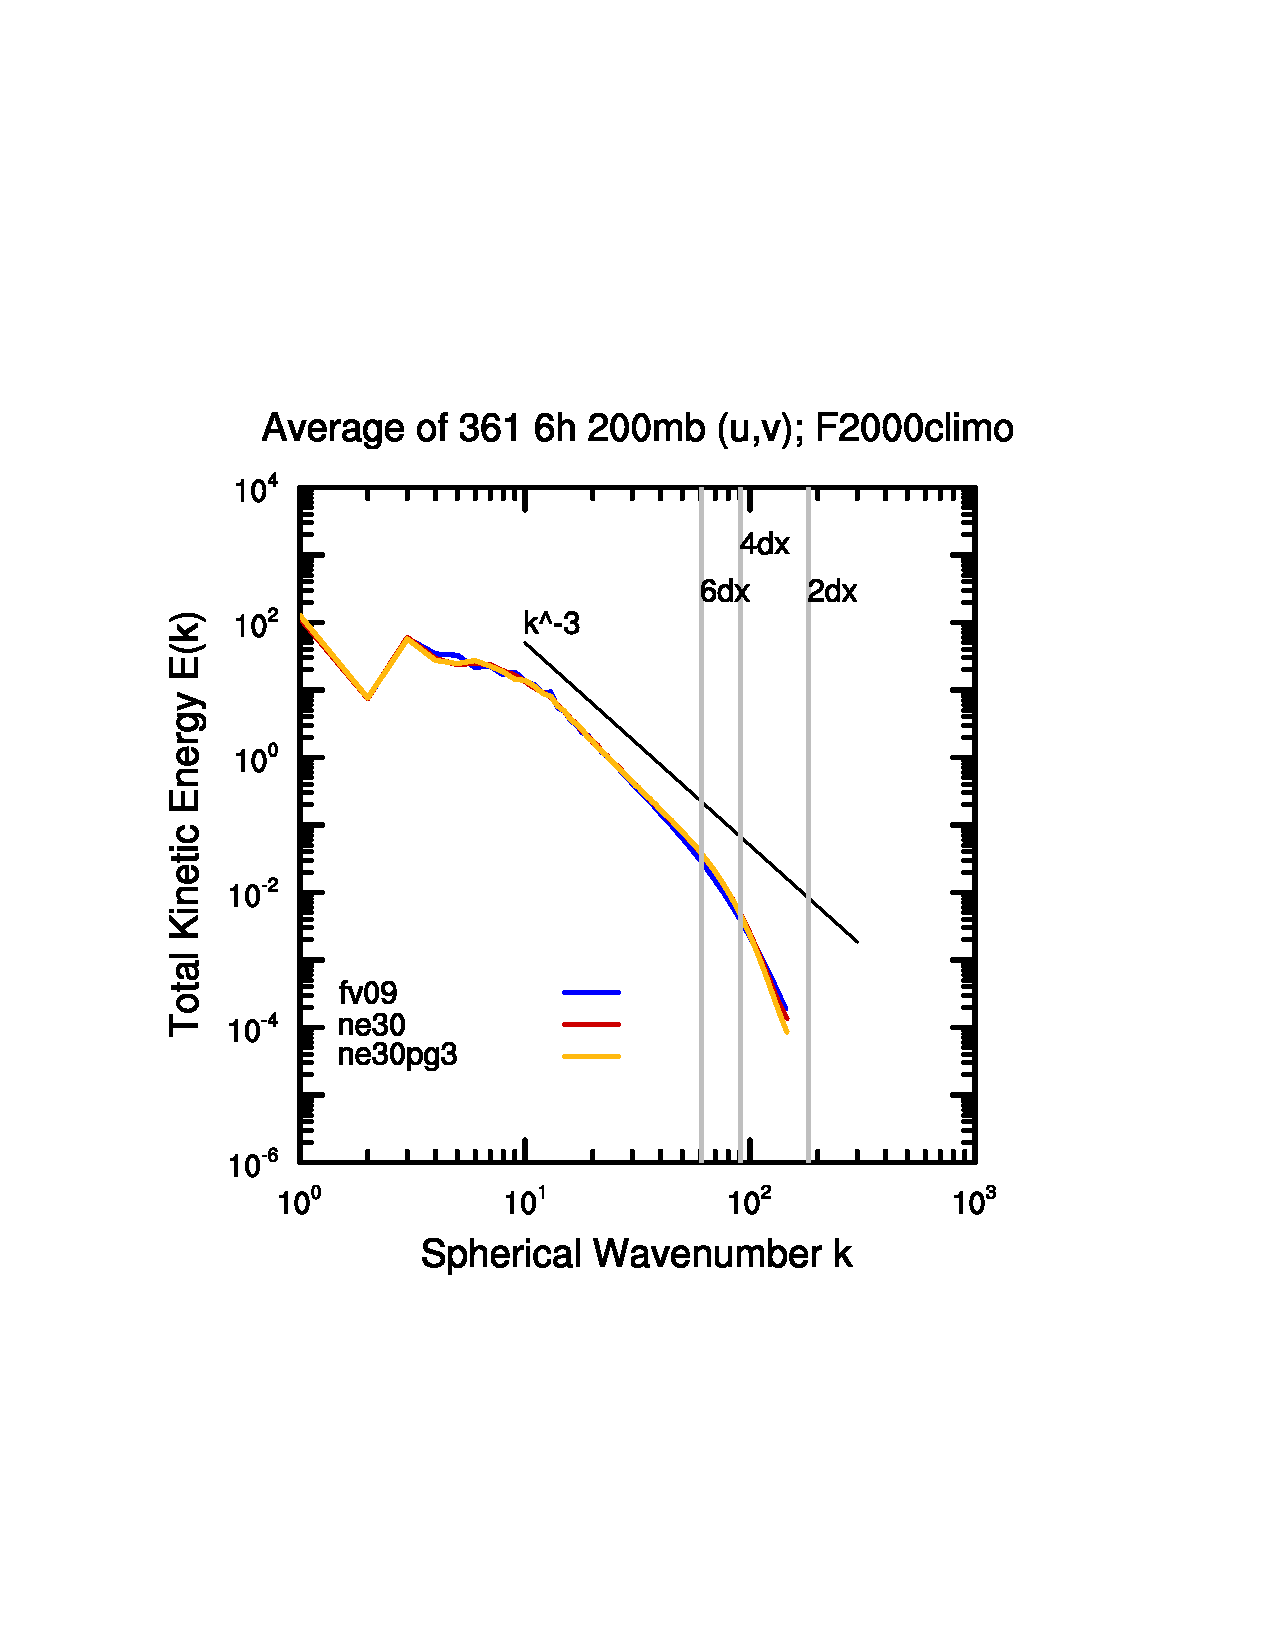
\includegraphics[width=\textwidth]{figs/tke.pdf}
\caption{Total kinetic energy spectrum of the horizontal winds at the 200-hPa level in CAM-FV (fv09), CAM-SE (ne30), CAM-SE-CSLAM (ne30pg3) and CAM-SE using CESM1.5 viscosity settings (ne30 CESM1.5) at approximately $1^\circ$ horizontal resolution , computed as the mean spectra from 30 days of 6-hourly instantaneous spectra. Black line is the $k^{-3}$ reference scaling, where $k$ is wavenumber. The grey vertical lines show approximately 6,4 and 2 wavelength $k$ values.}
\end{figure}

\subsubsection{Exner-based PGF (pressure gradient force)}
The PGF force formulation used in CESM1 is a standard formulation used in many legacy global climate models
\begin{equation}
\label{eq:pgf1}
 \nabla_{\eta^{(d)}} \Phi   + \frac{1}{\rho} \nabla_{\eta^{(d)}} p,
\end{equation}
where $\Phi$ is the geopotential height ($\Phi=g\, z$), $p$ pressure, $\rho$ density and $\eta^{(d)}$ is the dry-mass hybrid-sigma vertical coordinate. Significant improvement in the flow over topography can be achieved by using the Exner function 
\begin{equation}
\Pi \equiv \left( \frac{p}{p_0}\right)^{\frac{R^{(d)}}{c^{({d})}_p}},
\end{equation}
where $p_0=1000hPa$, $R^{(d)}$ is the gas constant for dry air and $c_p^{(d)}$ the heat capacity at constant pressure for dry air. The resulting PGF formula is 
\begin{equation}\label{eq:pgf2}
    \nabla_{\eta^{(d)}}\Phi+c_p^{(d)}\theta_v\nabla_{\eta^{(d)}}\Pi.
\end{equation}
where virtual potential temperature is
\begin{equation}
\theta_v\equiv \frac{T_v}{\Pi}
\end{equation}
and virtual temperature is given in equation (16) in \citeA{LetAl2018JAMES}. The derivation showing that (\ref{eq:pgf1}) and (\ref{eq:pgf2}) are equivalent is shown here:
\begin{eqnarray*}
c_p^{(d)}\theta_v\nabla_{\eta^{(d)}}\Pi &=& c_p^{(d)}\theta_v\nabla_{\eta^{(d)}}\left( \frac{p}{p_0}\right)^{\kappa},\\
&=& c_p^{(d)}\theta_v\kappa\left( \frac{p}{p_0}\right)^{\kappa-1} \nabla_{\eta^{(d)}}\left( \frac{p}{p_0}\right),\\
&=& c_p^{(d)}\theta_v\kappa\Pi\left( \frac{p_0}{p}\right) \nabla_{\eta^{(d)}}\left(\frac{p}{p_0}\right),\\
&=& \frac{c_p^{(d)}\theta_v\kappa\Pi}{p} \nabla_{\eta^{(d)}}p,\\
&=& \frac{R_d\theta_v\Pi}{p} \nabla_{\eta^{(d)}}p,\\
&=& \frac{R_dT_v}{p} \nabla_{\eta^{(d)}}p,\\
&=& \frac{1}{\rho} \nabla_{\eta^{(d)}}p.
\end{eqnarray*}
The Exner-based PGF formulation is used in a number of state-of-the-art models \cite <e.g.> {joyOfUM}.
\subsubsection{Reference profiles for viscosity}
Horizontal diffusion in terrain following coordinates is most conveniently performed on model levels, i.e. along $\eta^{(d)}$ coordinate surface in SE. When applied to temperature $T$, for example, there is a tendency to warm the atmosphere at higher ground where the coordinate surfaces slope steeply. This problem may be alleviated by applying diffusion operators to a variable the varies more uniformly with height. An approach, proposed by \citeA{SJ1991QJRMS}, is to subtract a static reference profile from temperature before applying the hyperviscosity operator
\begin{equation}
\nabla^4_{\eta^{(d)}}\left( T-T^{ref}\right),
\end{equation}
where
\begin{equation}
T^{ref}=
\end{equation}


In areas of steep terrain diffusion operators can tend to smooth


\subsubsection{Tuning of viscosity coefficients}
Our main goals during this tuning process was:
\begin{itemize}
\item use the same level of smoothing of topography as in CAM-FV
\item to reduce obvious noise in $\omega$ near steep terrain while not increasing explicit damping coefficients excessively
\item make sure model was stable in full physics configurations; the WACCM model is the most difficult to keep stable so a stable WACCM simulation capability was part of the testing
\end{itemize}

, to produce physical solutions for flow over steep topography. At the very least a physical solution is defined as a solution which is clearly {\em{not noisy}}. 

Unfortunately there does not seem to be a simplified standardized test case for such a tuning process wherefore we have developed our own.
[Held-Suarez topo]


[plot cross section of $T$; is their uphill warming without reference temperature?]
[see Mark's PPT; Download/hstopo.pptx]
\begin{itemize}
\item Switching to Exner pressure and prognostic potential temperature substantially reduces pressure gradient errors  (Thuburn, QJRMS, 2006; Toy \& Randall, JCP 2007)
\item Adjusting hyperviscosity to not dissipate hydrostatic background state further improves results near the surface
\end{itemize}


\subsection{Sponge layer damping for middle atmosphere models}
[The purpose of a numerical sponge is to damp vertical propagating from There are many choices in sponge layer damping. They can be divided into what the damping operator is (implicit or explicit) and what the vertical profile of the damping should be. In CAM-SE the sponge layer damping is explicit; Laplacian damping of the prognostic variables. Using that approach the vertical profile of the damping must be chosen. 

Reference ECWMF report

Why molecular and thermal? Vertical profile only depends on one parameter (strength) and not others as the TANH profile

Where in the atmosphere sponge is matters too? The higher the top the more the vertical waves will have grown in amplitude and the stronger the sponge layers needs to be!]

\subsubsection{Traditional sponge layer formulation}
\subsubsection{Molecular viscosity}
The 2D equation for molecular viscosity is
\begin{equation}
    \frac{du}{dt}=\frac{1}{\rho}\nabla_z \left( kmvis \nabla_z u\right),
\end{equation}
where $kmvis$ is dynamic viscosity coefficient which dependends on temperature and the composition of dry air [hanli: do you have a reference] (defined in CAM subroutine \verb+src/utils/physconst.F90+). Assuming a fixed trospheric composition of air then $kmvis$ is given by
\begin{equation}
..
\end{equation}
\begin{figure}
\noindent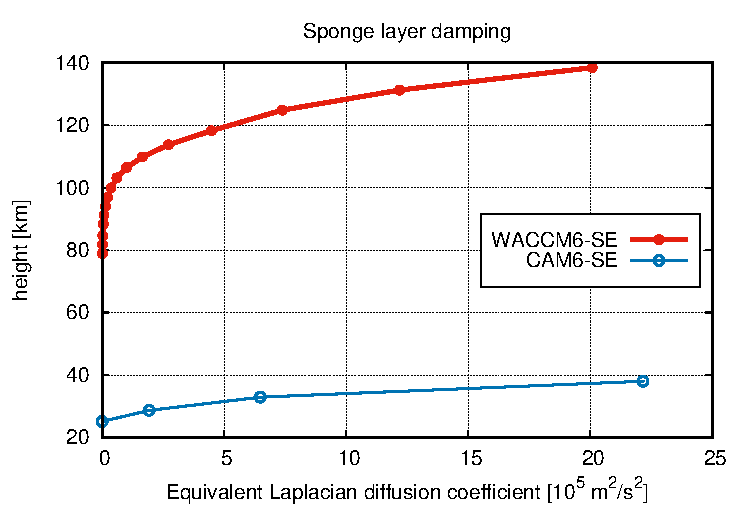
\includegraphics[width=\textwidth]{figs/sponge.pdf}
\caption{}
\end{figure}


The chain rule to convert to pressure coordinates is
\begin{equation}
    \nabla_p u=\nabla_z u +\left( \frac{\partial p}{\partial z}\right) \left( \nabla_p z\right)\left(\frac{\partial u}{\partial p}\right),
\end{equation}
Using the hydrostatic relation
\begin{equation}
    \frac{\partial p}{\partial z}=-\rho g,
\end{equation}
we get
\begin{equation}\label{eq:nablaz}
   \nabla_z u= \nabla_p u+\rho \nabla_p \Phi  \left(\frac{\partial u}{\partial p}\right).
\end{equation}
Maybe the second term on the right-hand side of (\ref{eq:nablaz}) is very small compared to the first term?
\subsection{Vertical}
The molecular diffusion equation for momentum components in the vertical is
\begin{equation}
    \frac{du}{dt}=\frac{1}{\rho}\frac{d}{dz}\left( kmvis \frac{du}{dz}\right).
\end{equation}
Changing to pressure coordinates yields
\begin{equation}
    \frac{du}{dt}=g^2\frac{d}{dp}\left( kmvis \, \rho\frac{du}{dp}\right).
\end{equation}
This means that the viscosity coefficient ($\nu$) used in the dynamical core is $g^2 \, kmvis \, \rho$.
\section{Thermal conductivity}
Similar to molecular viscosity except for $c_p$ term in equations
\begin{equation}
    \frac{d}{dt}\left( c_pT\right)=\frac{1}{\rho}\nabla_z \left( kmcnd \nabla_z T\right),
\end{equation}
and
\begin{equation}
    \frac{d}{dt}\left( c_pT\right)=\frac{1}{\rho}\frac{d}{dz}\left( kmcnd \frac{dT}{dz}\right).
\end{equation}
%%%%%%%%%%%%%%%%%%%%%%%%%%%%%%%%%%%%%%%%%%%%%%%%%%%%%%%%%%%%%%%%%%%%%%%%%%%%%%%%%%%%%%%%%%%%%%%%%%%%%%%%%%%%%%%%%%

\subsection{Pressure gradient force (PGF)}
The pressure gradient force discretization in CESM2.0 was based on the 
\begin{equation}
\nabla_{\eta^{(d)}} \Phi + \frac{1}{\rho} \nabla_{\eta^{(d)}} p,
\end{equation}
where $p$ is pressure, $\rho$ is density and $\Phi$ the geopotential. Significant reduction in the amount of grid-scale noise (in particular at element edges) in vertical down and updrafts near steep terrain can be achieved by switching to an Exner pressure formulation of the PGF ...



%
%https://github.com/E3SM-Project/E3SM/compare/master...mt5555:preqx-exner
%
%Mark: potential temperature in the thermodynamic equation does not make a difference.
%
%Biggest impact is Exner pressure in PGF
%Next is reference dp and T for viscosity

\subsection{Vertical remapping}
\begin{itemize}
\item water species, momentum and temperature are mapped using same method
\item this consistency is important (e.g. isothermal profile will not remain isothermal if water species are mapped with a method different than temperature)
\item non-water tracers are advected with exactly linear and shape-preserving scheme as in CESM2.0.
\end{itemize}
\subsection{Smoothing topography for variable resolution applications}
The topography boundary condition for variable resolution grids need to be smoothed in a way as to not excite grid-scale features, while also preserving the topographic steepness permitted in the refined regions. That is, the amount of smoothing applied to the raw elevation dataset should be larger for the coarse regions than in the refined regions. The NCAR global model topography generation software \cite{LetAl2015GMD} has been updated to include differential smoothing that depends on the local spectral-element area, described here. 

The topography software uses a two step process to generate the topography for a given target grid. It first takes a global high-resolution (1km) elevation dataset and maps the elevations to an unstructured cubed-sphere grid with a 3km horizontal resolution. This step is no different whether a uniform or variable-resolution grid. The second step smoothes the elevations on the 3km grid and then maps the smoothed field to the target grid. The radius of the smoothing kernel is a free parameter that needs to be adjusted depending on the target grid resolution. CESM uses a smoothing radius of about twice the grid spacing of the target grid. For example, a uniform resolution $1^{\circ}$ grid uses a 60 point radius on the 3km cubed-sphere grid. For variable resolution grids, a refinement factor is defined on the target grid, and mapped to the 3km cubed-sphere grid to inform the smoothing radius. Arriving at a refinement factor on the 3km cubed-sphere is a four step process:
\begin{itemize}
\item Compute the element area $A_{elem}$ on the computational grid.
\item Use this area to define a refinement factor on the computational grid $\sqrt{\frac{MAX(A_{elem})}{A_{elem}}}$.
\item Remap the refinement factor to the 3km cubed-sphere, $rrfac_{cube}$.
\item Smooth $rrfac_{cube}$ using a kernel radius 4 times that used to smooth terrain in the coarse regions.
\item Round $rrfac_{cube}$ to the nearest integer, and limit values to be no larger than $rrfac_{max}$.
\end{itemize}

The smoothing radius $R$ applied to the terrain in variable resolution grids varies over the grid by setting it to $R=\frac{R_{0}}{rrfac_{cube}}$, where $R_0$ is the smoothing radius used in the coarse region.

\subsection{Code stuff: generalized thermodynamic code}
\begin{itemize}
\item utils/physconst.F90: unify new code for {\em{kmvis}} and {\em{kmcnd}} for WACCM-x. Similarly for heat capacity and R.
\end{itemize}
\section{Results}
\subsection{CAM}
[what CAM results should we show]
\subsection{Support for CONUS and Arctic variable resolution grids}
There are many studies using CESM in a variable-resolution configuration (VR-CESM) with the CAM-SE dynamical core. These studies were performed in collaboration with variable-resolution specialists whose time and resources are limited and not available to the broader community. CESM2.2 provides functional support for three variable-resolution grids in CAM-SE that is easily configured and can be ran by any user. These are the ARCTIC, ARCTICGRIS and CONUS grids depicted in Figure~X. The ARCTIC grid has uniform base resolution of $1^{\circ}$ with $\frac{1}{4}^{\circ}$ refinement over the broader Arctic. The ARCTICGRIS grid is identical to the ARCTIC grid but contains an additional $\frac{1}{8}^{\circ}$ refined patch over Greenland. The CONUS grid has a $1^{\circ}$ base resolution with $\frac{1}{8}^{\circ}$ refinement covering the contiguous U.S. An earlier iteration of the CONUS grid has been described in a prior study \cite{GetAl2017JAMES}. The CONUS grid described here is central to the debut of the Mulit-Scale Infrastructure for Chemistry and Aerosols for use in atmospheric chemistry studies \cite{MUSICA2020}.

\subsection{WACCM QBO}
Quasi-biennial Oscillation (QBO) is a prominent feature of the tropical stratosphere. The QBO is very difficult to represent in GCMs, for example, only 3 out of 27 CMIP5 models had an internally generated QBO. Necessary processes to simulate accurately for a successful simulation of the QBO is resolved Kelvin and mixed-Rossby gravity waves and small-scale gravity waves (which are parameterized in WACCM: Beres et al. 2002, Richter et al. 2010). To achieve this adequate vertical resolution is necessary. The finite-volume dynamical core with 110 vertical levels has successfully simulated the QBO [ref].

\begin{itemize}
\item show that vertical remapping method matters for 70 layer model
\item tuning needed \verb+effgw_beres+
\end{itemize}
\begin{figure}
\noindent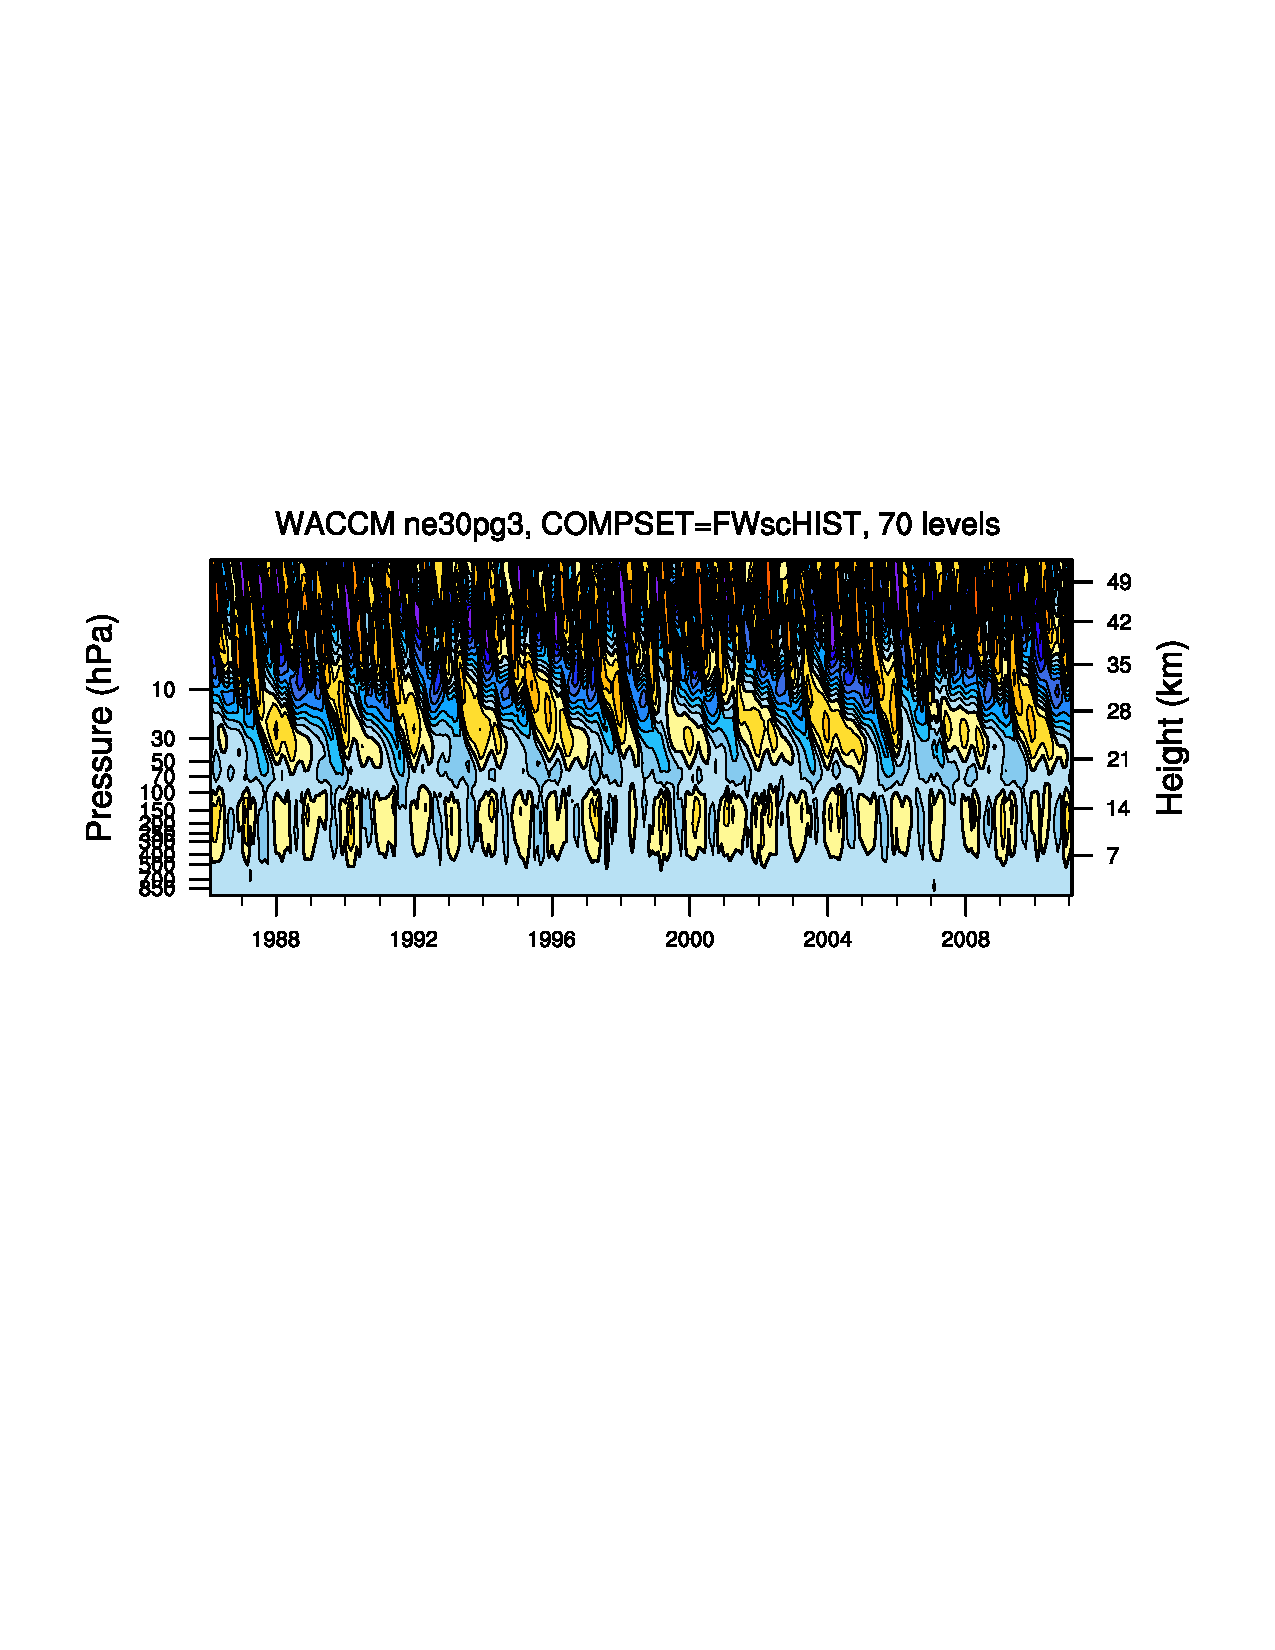
\includegraphics[width=\textwidth]{figs/FWscHIST-nlev70.pdf}
\noindent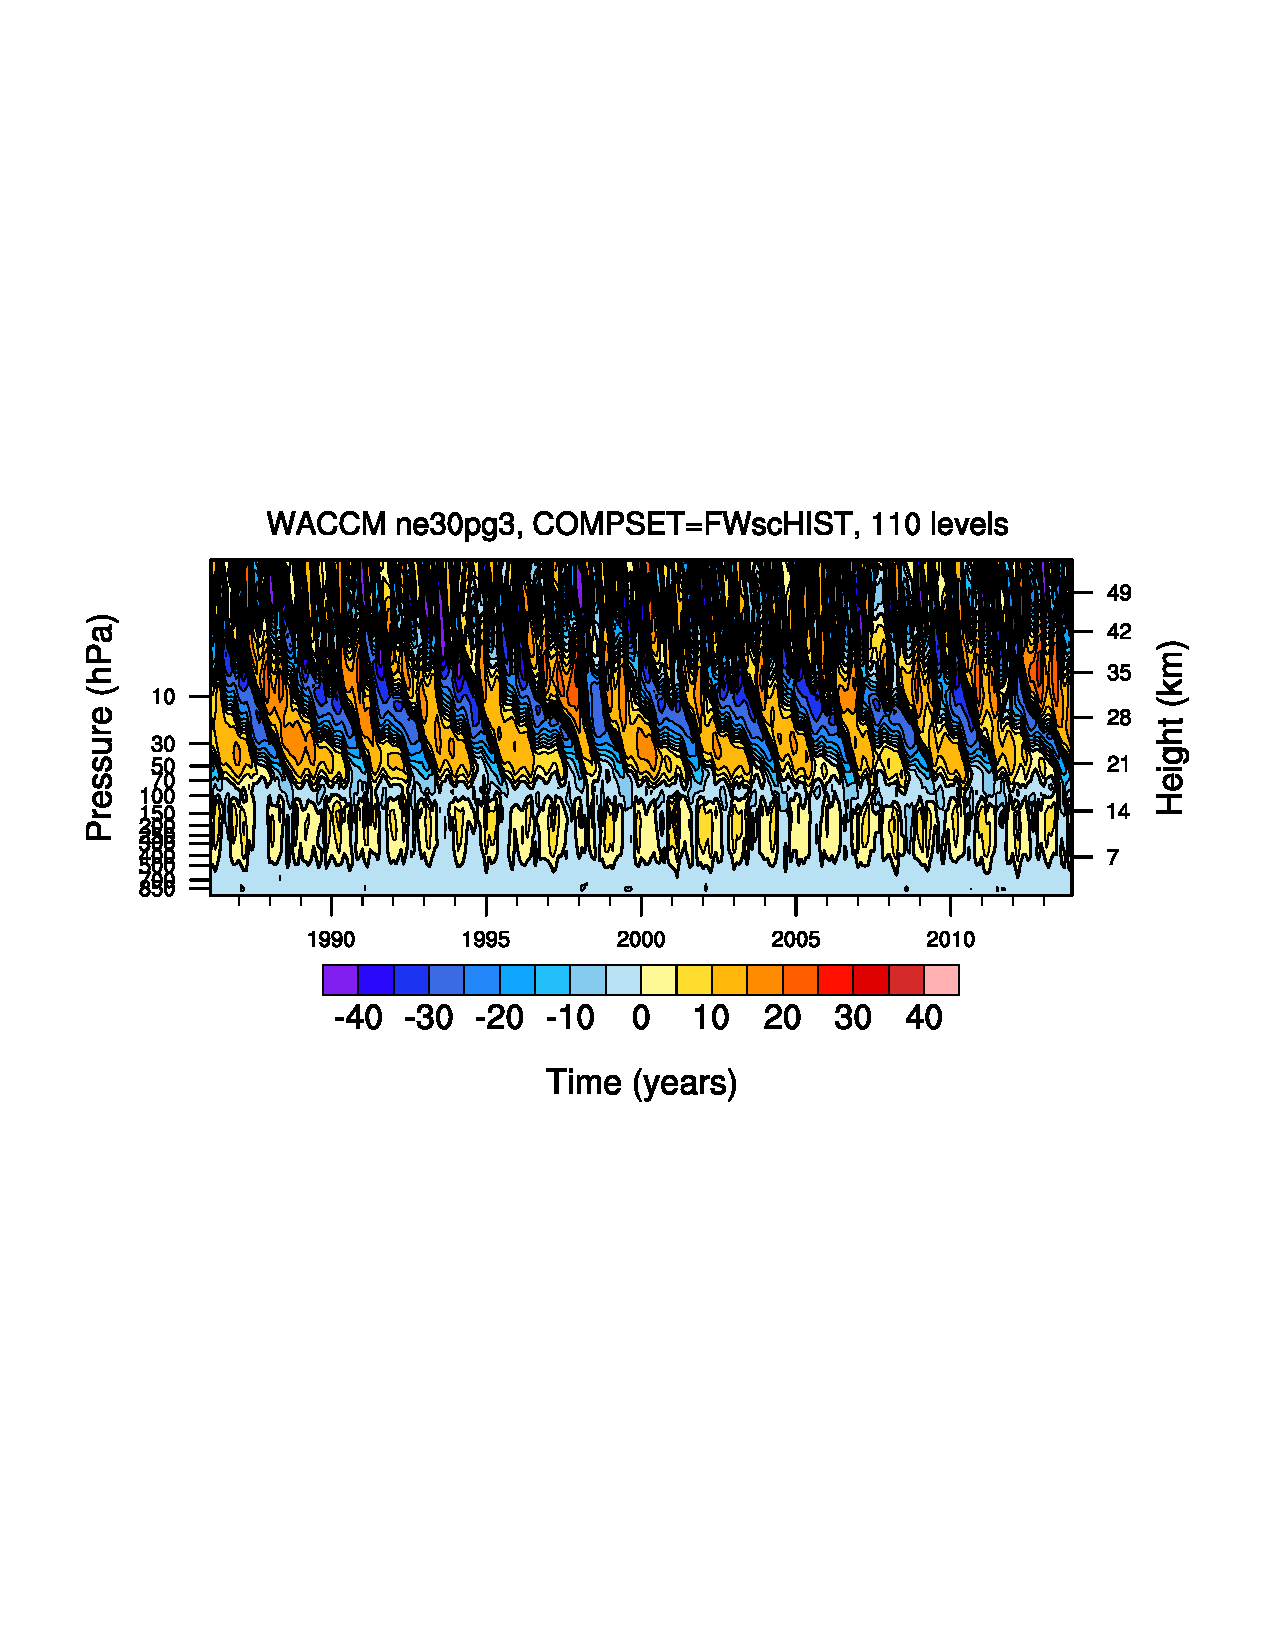
\includegraphics[width=\textwidth]{figs/FWscHIST-nlev110.pdf}
\caption{[warning: these figures are not final] Tropical zonal winds ($2^\circ S$ to $2^\circ N$ average) simulated in historical simulation using approximately 1 degree SE-CSLAM with (upper plot) 70 and (lower plot) 110  levels in the vertical, respectively.}
\end{figure}
\subsection{ACOM CONUS result?}
\subsection{Performance: CAM and WACCM}
[check with John] [remember pcols setting for pecount 5400]

\begin{itemize}
\item verb+FWsc2000+ (41 tracers): SYPD = 4.825 (ne30) and SYPD = 5.763 (ne30pg3); 1 month test with interpolated monthly output.=> 19% faster
\item verb+FW2000+ (201 tracers): SYPD =  1.171 (ne30) and SYPD = 1.655 (ne30pg3); 5 day run => 40% faster [verify these numbers!]
\item verb+FW2000+ (201 tracers), CONUS: 11-12 days in 12 hours using 5400 PEs
\begin{verbatim}
                         ne30      ne30pg3
prim_advec_tracers_fvm             358.263
prim_advec_tracers_remap 682.674   19.256
vertical_remap            37.047   43.460
dp_couling                16       16.7
p_d_coupling              23       29
\end{verbatim}


\end{itemize}
% \section{Materials and Methods}
% Here is text on Materials and Methods.
%
% \subsection{A descriptive heading about methods}
% More about Methods.
%
% \section{Data} (Or section title might be a descriptive heading about data)
%
% \section{Results} (Or section title might be a descriptive heading about the
% results)
%

\section{Conclusions}

\section{Things to do before release [not included in final manuscript!]}
\subsection{Initial condition files}
\begin{itemize}
\item \verb+ne30pg4+ WACCM initial condition (with and without chemistry)
\item CAM initial condition from John's runs
\item CONUS WACCM initial condition (with chemistry)
\end{itemize}
\subsection{physconst.F90}
\begin{itemize}
\item species dependent code
\end{itemize}
\subsection{clean-up}
\begin{itemize}
\item remove namelist options that are not tested: variable\_nsplit, ...
\end{itemize}
\subsection{check}
\begin{itemize}
\item do we have tracer distributions for tracer tests?
\item can we add 3 tracer test from QJRMS paper?
\end{itemize}
\section{= enter section title =}
%Text here ===>>>


%%

%  Numbered lines in equations:
%  To add line numbers to lines in equations,
%  \begin{linenomath*}
%  \begin{equation}
%  \end{equation}
%  \end{linenomath*}



%% Enter Figures and Tables near as possible to where they are first mentioned:
%
% DO NOT USE \psfrag or \subfigure commands.
%
% Figure captions go below the figure.
% Table titles go above tables;  other caption information
%  should be placed in last line of the table, using
% \multicolumn2l{$^a$ This is a table note.}
%
%----------------
% EXAMPLE FIGURES
%
% \begin{figure}
% \includegraphics{example.png}
% \caption{caption}
% \end{figure}
%
% Giving latex a width will help it to scale the figure properly. A simple trick is to use \textwidth. Try this if large figures run off the side of the page.
% \begin{figure}
% \noindent\includegraphics[width=\textwidth]{anothersample.png}
%\caption{caption}
%\label{pngfiguresample}
%\end{figure}
%
%
% If you get an error about an unknown bounding box, try specifying the width and height of the figure with the natwidth and natheight options. This is common when trying to add a PDF figure without pdflatex.
% \begin{figure}
% \noindent\includegraphics[natwidth=800px,natheight=600px]{samplefigure.pdf}
%\caption{caption}
%\label{pdffiguresample}
%\end{figure}
%
%
% PDFLatex does not seem to be able to process EPS figures. You may want to try the epstopdf package.
%

%
% ---------------
% EXAMPLE TABLE
%
% \begin{table}
% \caption{Time of the Transition Between Phase 1 and Phase 2$^{a}$}
% \centering
% \begin{tabular}{l c}
% \hline
%  Run  & Time (min)  \\
% \hline
%   $l1$  & 260   \\
%   $l2$  & 300   \\
%   $l3$  & 340   \\
%   $h1$  & 270   \\
%   $h2$  & 250   \\
%   $h3$  & 380   \\
%   $r1$  & 370   \\
%   $r2$  & 390   \\
% \hline
% \multicolumn{2}{l}{$^{a}$Footnote text here.}
% \end{tabular}
% \end{table}

%% SIDEWAYS FIGURE and TABLE
% AGU prefers the use of {sidewaystable} over {landscapetable} as it causes fewer problems.
%
% \begin{sidewaysfigure}
% \includegraphics[width=20pc]{figsamp}
% \caption{caption here}
% \label{newfig}
% \end{sidewaysfigure}
%
%  \begin{sidewaystable}
%  \caption{Caption here}
% \label{tab:signif_gap_clos}
%  \begin{tabular}{ccc}
% one&two&three\\
% four&five&six
%  \end{tabular}
%  \end{sidewaystable}

%% If using numbered lines, please surround equations with \begin{linenomath*}...\end{linenomath*}
%\begin{linenomath*}
%\begin{equation}
%y|{f} \sim g(m, \sigma),
%\end{equation}
%\end{linenomath*}

%%% End of body of article

%%%%%%%%%%%%%%%%%%%%%%%%%%%%%%%%
%% Optional Appendix goes here
%
% The \appendix command resets counters and redefines section heads
%
% After typing \appendix
%
%\section{Here Is Appendix Title}
% will show
% A: Here Is Appendix Title
%
%\appendix
%\section{Here is a sample appendix}

%%%%%%%%%%%%%%%%%%%%%%%%%%%%%%%%%%%%%%%%%%%%%%%%%%%%%%%%%%%%%%%%
%
% Optional Glossary, Notation or Acronym section goes here:
%
%%%%%%%%%%%%%%
% Glossary is only allowed in Reviews of Geophysics
%  \begin{glossary}
%  \term{Term}
%   Term Definition here
%  \term{Term}
%   Term Definition here
%  \term{Term}
%   Term Definition here
%  \end{glossary}

%
%%%%%%%%%%%%%%
% Acronyms
%   \begin{acronyms}
%   \acro{Acronym}
%   Definition here
%   \acro{EMOS}
%   Ensemble model output statistics
%   \acro{ECMWF}
%   Centre for Medium-Range Weather Forecasts
%   \end{acronyms}

%
%%%%%%%%%%%%%%
% Notation
%   \begin{notation}
%   \notation{$a+b$} Notation Definition here
%   \notation{$e=mc^2$}
%   Equation in German-born physicist Albert Einstein's theory of special
%  relativity that showed that the increased relativistic mass ($m$) of a
%  body comes from the energy of motion of the body—that is, its kinetic
%  energy ($E$)—divided by the speed of light squared ($c^2$).
%   \end{notation}




%%%%%%%%%%%%%%%%%%%%%%%%%%%%%%%%%%%%%%%%%%%%%%%%%%%%%%%%%%%%%%%%
%
%  ACKNOWLEDGMENTS
%
% The acknowledgments must list:
%
% >>>>	A statement that indicates to the reader where the data
% 	supporting the conclusions can be obtained (for example, in the
% 	references, tables, supporting information, and other databases).
%
% 	All funding sources related to this work from all authors
%
% 	Any real or perceived financial conflicts of interests for any
%	author
%
% 	Other affiliations for any author that may be perceived as
% 	having a conflict of interest with respect to the results of this
% 	paper.
%
%
% It is also the appropriate place to thank colleagues and other contributors.
% AGU does not normally allow dedications.


\acknowledgments
This material is based upon work supported by the National Center for Atmospheric Research (NCAR), which is a major facility sponsored by the NSF under Cooperative Agreement 1852977. Computing and data storage resources, including the Cheyenne supercomputer
(doi:10.5065/D6RX99HX), were provided by the Computational and Information Systems Laboratory (CISL) at NCAR.

The data presented in this manuscript is available at {\url{https://github.com/PeterHjortLauritzen/CESM2.2.git}}.



%% ------------------------------------------------------------------------ %%
%% References and Citations

%%%%%%%%%%%%%%%%%%%%%%%%%%%%%%%%%%%%%%%%%%%%%%%
%
% \bibliography{<name of your .bib file>} don't specify the file extension
%
% don't specify bibliographystyle
%%%%%%%%%%%%%%%%%%%%%%%%%%%%%%%%%%%%%%%%%%%%%%%

%\bibliography{ enter your bibtex bibliography filename here }
\bibliography{bib}


%Reference citation instructions and examples:
%
% Please use ONLY \cite and \citeA for reference citations.
% \cite for parenthetical references
% ...as shown in recent studies (Simpson et al., 2019)
% \citeA for in-text citations
% ...Simpson et al. (2019) have shown...
%
%
%...as shown by \citeA{jskilby}.
%...as shown by \citeA{lewin76}, \citeA{carson86}, \citeA{bartoldy02}, and \citeA{rinaldi03}.
%...has been shown \cite{jskilbye}.
%...has been shown \cite{lewin76,carson86,bartoldy02,rinaldi03}.
%... \cite <i.e.>[]{lewin76,carson86,bartoldy02,rinaldi03}.
%...has been shown by \cite <e.g.,>[and others]{lewin76}.
%
% apacite uses < > for prenotes and [ ] for postnotes
% DO NOT use other cite commands (e.g., \citet, \citep, \citeyear, \nocite, \citealp, etc.).
%



\end{document}



More Information and Advice:

%% ------------------------------------------------------------------------ %%
%
%  SECTION HEADS
%
%% ------------------------------------------------------------------------ %%

% Capitalize the first letter of each word (except for
% prepositions, conjunctions, and articles that are
% three or fewer letters).

% AGU follows standard outline style; therefore, there cannot be a section 1 without
% a section 2, or a section 2.3.1 without a section 2.3.2.
% Please make sure your section numbers are balanced.
% ---------------
% Level 1 head
%
% Use the \section{} command to identify level 1 heads;
% type the appropriate head wording between the curly
% brackets, as shown below.
%
%An example:
%\section{Level 1 Head: Introduction}
%
% ---------------
% Level 2 head
%
% Use the \subsection{} command to identify level 2 heads.
%An example:
%\subsection{Level 2 Head}
%
% ---------------
% Level 3 head
%
% Use the \subsubsection{} command to identify level 3 heads
%An example:
%\subsubsection{Level 3 Head}
%
%---------------
% Level 4 head
%
% Use the \subsubsubsection{} command to identify level 3 heads
% An example:
%\subsubsubsection{Level 4 Head} An example.
%
%% ------------------------------------------------------------------------ %%
%
%  IN-TEXT LISTS
%
%% ------------------------------------------------------------------------ %%
%
% Do not use bulleted lists; enumerated lists are okay.
% \begin{enumerate}
% \item
% \item
% \item
% \end{enumerate}
%
%% ------------------------------------------------------------------------ %%
%
%  EQUATIONS
%
%% ------------------------------------------------------------------------ %%

% Single-line equations are centered.
% Equation arrays will appear left-aligned.

Math coded inside display math mode \[ ...\]
 will not be numbered, e.g.,:
 \[ x^2=y^2 + z^2\]

 Math coded inside \begin{equation} and \end{equation} will
 be automatically numbered, e.g.,:
 \begin{equation}
 x^2=y^2 + z^2
 \end{equation}


% To create multiline equations, use the
% \begin{eqnarray} and \end{eqnarray} environment
% as demonstrated below.
\begin{eqnarray}
  x_{1} & = & (x - x_{0}) \cos \Theta \nonumber \\
        && + (y - y_{0}) \sin \Theta  \nonumber \\
  y_{1} & = & -(x - x_{0}) \sin \Theta \nonumber \\
        && + (y - y_{0}) \cos \Theta.
\end{eqnarray}

%If you don't want an equation number, use the star form:
%\begin{eqnarray*}...\end{eqnarray*}

% Break each line at a sign of operation
% (+, -, etc.) if possible, with the sign of operation
% on the new line.

% Indent second and subsequent lines to align with
% the first character following the equal sign on the
% first line.

% Use an \hspace{} command to insert horizontal space
% into your equation if necessary. Place an appropriate
% unit of measure between the curly braces, e.g.
% \hspace{1in}; you may have to experiment to achieve
% the correct amount of space.


%% ------------------------------------------------------------------------ %%
%
%  EQUATION NUMBERING: COUNTER
%
%% ------------------------------------------------------------------------ %%

% You may change equation numbering by resetting
% the equation counter or by explicitly numbering
% an equation.

% To explicitly number an equation, type \eqnum{}
% (with the desired number between the brackets)
% after the \begin{equation} or \begin{eqnarray}
% command.  The \eqnum{} command will affect only
% the equation it appears with; LaTeX will number
% any equations appearing later in the manuscript
% according to the equation counter.
%

% If you have a multiline equation that needs only
% one equation number, use a \nonumber command in
% front of the double backslashes (\\) as shown in
% the multiline equation above.

% If you are using line numbers, remember to surround
% equations with \begin{linenomath*}...\end{linenomath*}

%  To add line numbers to lines in equations:
%  \begin{linenomath*}
%  \begin{equation}
%  \end{equation}
%  \end{linenomath*}



